\documentclass{llncs}
\usepackage{subcaption}
\usepackage{subfig} 
\usepackage{usual}
\usepackage{graphicx}
\usepackage[rflt]{floatflt}
\usepackage{multirow}
\pagestyle{plain} 

\begin{document}
\title{\vskip -10pt Pilot study}

\author{Lydia Ould Ouali\inst{1}, Charles Rich\inst{2} \and
Nicolas Sabouret\inst{1} }

\institute{LIMSI-CNRS, UPR 3251, Orsay, France \\
Universit\'e Paris-Sud, Orsay, France \\
\email{\{ouldouali, nicolas.sabouret\}@limsi.fr}
\and
Worcester Polytechnic Institute\\ Worcester, Massachusetts, USA\\
\email{rich@wpi.edu}
}
\maketitle 


\section{Experimental design}
We built a model of dialogue which is capable to have a cooperative negotiation with a user. Moreover, we allow our system to adapt its negotiation strategy in function to the perceived relation of dominance with the other. 
In order to understand better how the dominance behavior can appear in the dialogue, we conducted an experiment in which we asked participants to read dialogues generated with our model.  


The model produces a dialogue of cooperative negotiation where two agents have to decide in which restaurant they will go dinner. The behavior of each agent is affected by its perception of his relation of dominance with the other agent.

Behaviors related to dominance were generated following principals related in social psychology. We kept three principals of verbal behaviors: 
\begin{enumerate}
	\item Dominant negotiator tends to not pay attention to the other negotiator and is only concerned by satisfying its preferences. While, submissive negotiator is dependent and take in consideration the other negotiator preferences to make a decision. \cite{van2006power}
	\item Dominant negotiator is very demanding and refuses to make concessions, while the submissive agent is more flexible. \cite{dreu1995impact}
	\item Dominant negotiator tends to take the control of the dialogue, in term of controlling the flow of the dialogue and orient the negotiation vice versa. \cite{galinsky2003power}
\end{enumerate}	
We designed our agents to follow three different behaviors of dominance:\textit{ dominant, submissive and a peer agent}. We generated two types of dialogues: dialogues in which agents have \textbf{unbalanced} relation of dominance (\textit{dominant} agent dialogues with submissive, and dialogues with \textbf{balanced} relation of dominance (two \textit{peer} agents). Because the preferences affect directly the flow of the negotiation, we initialized agents with different types of preferences model. For each dialogue, agents are initialized with either \textbf{similar} preferences or in the contrary \textbf{different} preferences that we reverse to observe for the same preferences how the relation of dominance changes the behavior of agents(see table\ref{table}). For example:
\begin{enumerate}
	\item \textit{Dialogue1: Dominant agent initialized with the model of preferences S1, and submissive agent initialized with the model of preferences S2.}
	\item \textit{Dialogue 2 which is the reverse of dialogue 1: Dominant agent initialized with the model of preferences S2, and submissive agent initialized with the model of preferences S1.}
\end{enumerate}
\begin{table}[h]
	\centering
	\begin{tabular}{|c|c|c|} 
		\hline
		Preferences models & Unbalanced relation & Balanced relation\\
		\hline
		Similar preferences & \{$S_1$,$S_2$\} & \{$S_1$,$S_2$\} \\
		\cline{2-3} 
		& \{$S_2$,$S_1$\} & \{$S_2$,$S_1$\} \\
		\hline
		Different preferences & \{$D_1$,$D_2$\} & \{$D_1$,$D_2$\} \\
		\cline{2-3} 
		& \{$D_2$,$D_1$\} & \{$D_2$,$D_1$\} \\
		\hline
	\end{tabular} 
		\caption{\label{table} parameters of dialogue generation}
\end{table}
We obtain at the end eight dialogues in which we aim to analyze how the behavior of each of three agents shows in a dialogue. Thus, three conditions we manipulated.
In \emph{condition 1}, we analyzed the dominant agent behavior during all the dialogues of unbalanced relation. In \emph{condition 2}, we analyzed the peer agent behavior for all the dialogues of balanced relation. In \emph{condition 3}, we analyzed the behavior of the submissive agents for all the dialogues of unbalanced relation.

\section{Hypotheses}
Agent behaviors were modeled based on three principals from existing social psychology theory. Based on these principals, we developed three hypotheses:

\begin{itemize}
	\item H1: \textbf{(a)-}Participants will perceive dominant agent as a self-centered.\textbf{(b)-} Peer agent will perceive as considering more the preferences of other than the dominant agent. \textbf{(c)-} Submissive agent will be perceived as more interested to the other preferences than the peer agent in decision making.
	\item H2: \textbf{(a)-} dominant agent is perceived as more demanding(less flexible) than other agents. \textbf{(b)-}Peer agent will be perceived as less flexible than the submissive agent. \textbf{(c)-} Submissive agent will perceived the most flexible agent.
	
	\item H3: \textbf{(a)-} Dominant agent is perceived as the leader of the dialogue. \textbf{(b)-} Peer agent is perceived as more leading the dialogue than the submissive agent. \textbf{(c)-} submissive agent  will be perceived as a follower.
	
\end{itemize}

\section{Experimental study}
We conducted a between-subjects experiment, with two dialogues. The first dialogue was set between a dominant agent and a submissive agent initialized with different preferences. The second dialogue concerns two peer agents with similar preferences. 


Participants were asked to read the dialogues. They answered next to a questionnaire that measures their perception of agent’s behaviors during the dialogue. 

For each hypothesis, we defined two questions that measure the participants review for each agent (See table). We had a total of 12 questions related to the relation of dominance.

\begin{table}[t]
	\centering
	\begin{tabular}{|c|l|} 
		\hline
		Principal & questionnaire item\\
		\hline
		 \multirow{2}{*}{Principal 1} & Agent considers only his/her own preferences in choosing a restaurant. \\ \cline{2-2}
		 							  & Agent takes into account the preferences of the other speaker in choosing a restaurant. \\
		\hline	
		\multirow{2}{*}{Principal 2} & Agent is flexible in the choice of the restaurant. \\ \cline{2-2}
									 & Agent is inflexible in the choice of the restaurant. \\ 
		\hline
		\multirow{2}{*}{Principal 3} & Agent leads the dialogue. \\ \cline{2-2}
									 &  Agent is being guided by the other speaker during the dialogue.\\ 
		\hline
	\end{tabular} 
	\caption{\label{table2} Questionnaire items}
\end{table}

The questionnaire also included  questions for manipulation check. For the first question we asked subjects which restaurant was chosen in the conversation. The second question was relative to agent's expressed preferences in the dialogue. Five-point Likert scales were used in all questionnaire items.

A total of 20 subjects participated to the experiment (10 per dialogue). We excluded 4 subjects who incorrectly answer to manipulation test questions. (1 for the first dialogue, and 3 for the second one).
\subsection{Statistical analysis}

We first collected the answers given by the subjects for each question, that we sorted by agent (dominant, peer, submissive). Therefore, for each agent type, we gathered subjects perception of the dominance behavior. For all the dialogues, we obtain for each question, 9 answers for dominant and submissive agents, and 14 answers for peer agent. 

\par To analyze behavioral data, we applied a T-student analysis for independent variables to compute if there is a significant difference among agents behavior for each question.  

\par As data was gathered from different dialogues, we consider them as independent variables for the T-student. However, for this experiment, data for the dominant and submissive agent were collected from the same dialogue. Thus we applied a paired T-student to compare the submissive and dominant agents.
In order to be able to compute the T-student, data must have a normal distribution. For the experiment, data don't follow a normal distribution due to small size of the sample.
We present the obtained results for each hypothesis, in which we calculated the average agreement for each question and the standard deviation.

\subsubsection{Hypothesis 1 }
The analysis showed that for the first question, there is no significant difference between agents behaviors (see fig 1.a). For all the cases p>0.05, even if in average subjects agree that the submissive agent consider the preferences of other in decision making more than the peer and dominant agents. While, for the second question (Reverse question), they highly agree that the dominant agent only consider its preferences (p = 0.01 for dominant Vs peer, p<0.001 for dominant Vs submissive), and the peer agent considers his preferences more than the submissive agent (p =0.01). 

\begin{figure}[t]
	\begin{subfigure}{2.3in}
		\centerline{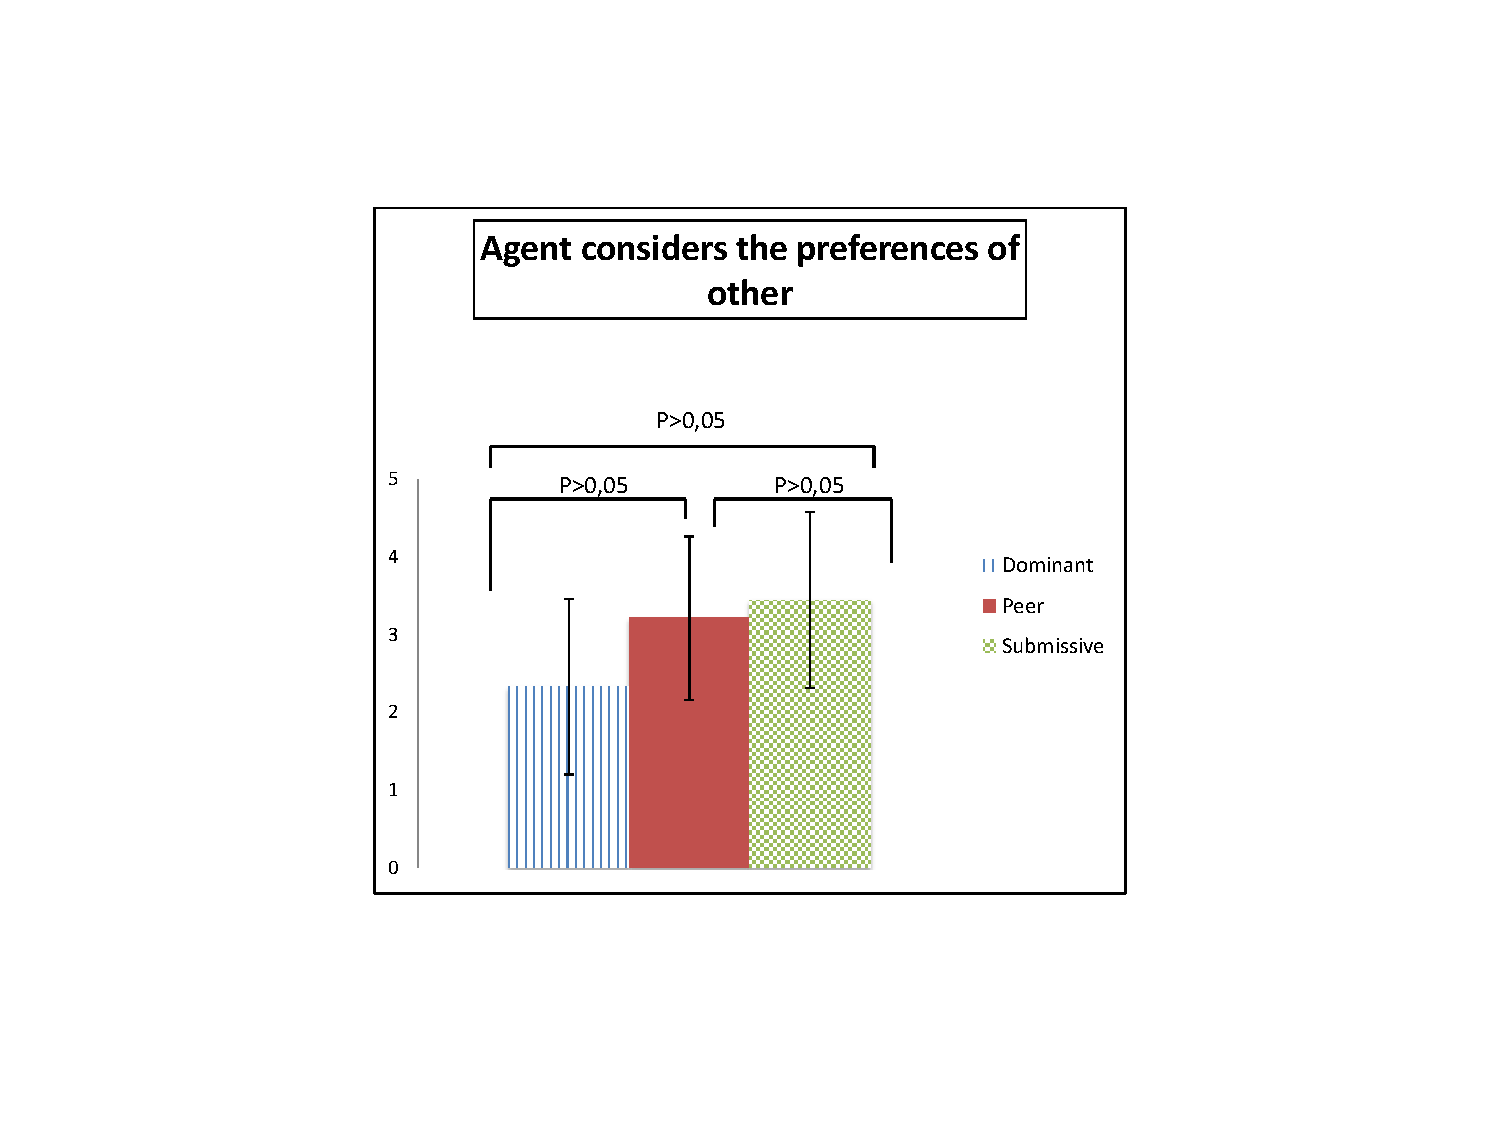
\includegraphics[width=2.4in]{figs/h1a}}
		\vskip 8pt 
		\defig{h1a}{a}
	\end{subfigure}
		\begin{subfigure}{2.3in}
			\centerline{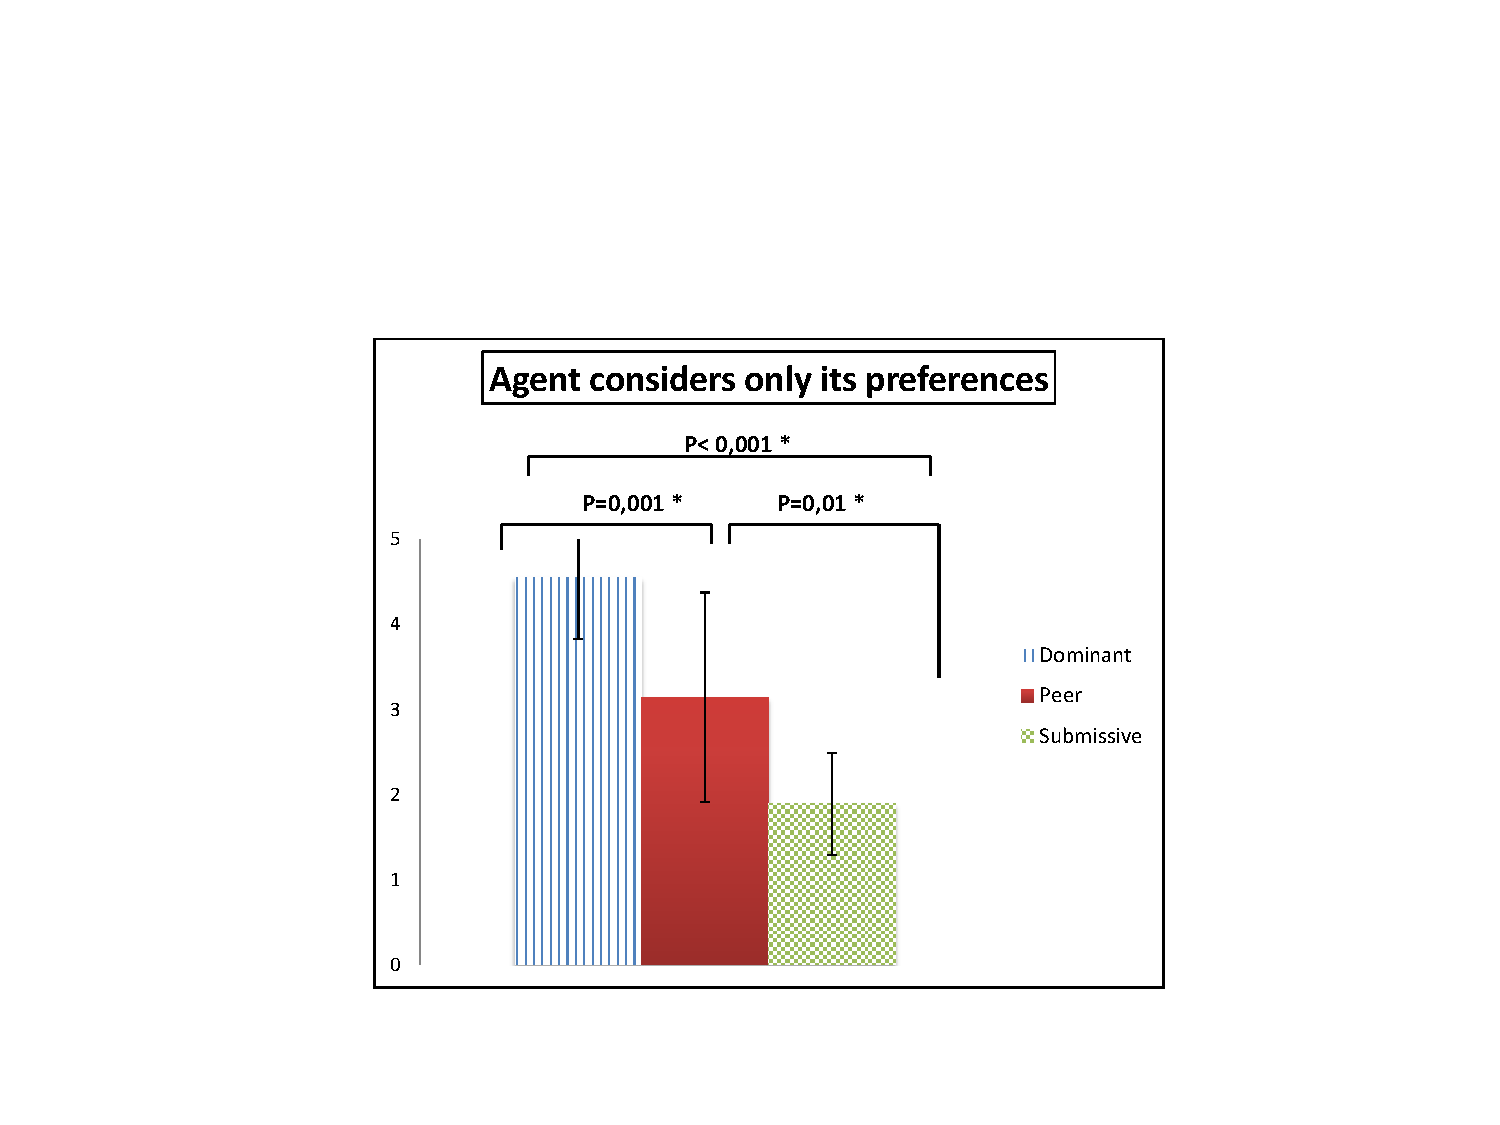
\includegraphics[width=2.5in]{figs/h1b}}
			\vskip 8pt 
			\defig{h1b}{b}
		\end{subfigure}
	\vskip 8pt
	\defig {h1}{Subjects rating for hypothesis 1}
\end{figure}
\bibliographystyle{plain}
\bibliography{abbrevs,Library}
\end{document}

\subsubsection{Hypothesis 2}
The results give support for only one question of the hypothesis H2. Indeed, for the question “agent is demanding” there was no significant difference observed among the three agent (for each case p>0.05). While for the reverse question, dominant agent was rated as being less flexible than the peer and submissive agent. This difference of perception between the two questions might be related to a wrong understanding to “the notion of demand” in the question in fig 2.a. 

\subsubsection{Hypothesis 3}
The analysis confirmed our third hypothesis. For the question “who leads the dialogue”, dominant agent was perceived as more leading the dialogue than the peer and the submissive agent (p=0.01) as presented in figure 3.a. In the contrary, submissive agent was perceived as being leaded in the dialogue compared to the dominant agent (p<0.01).  However, there is no significant difference between the Peer and the submissive agent as presented in figure 3.b.
\section{Discussion}